\documentclass[10pt, a4paper, spanish]{article}
\usepackage[paper=a4paper, left=1.5cm, right=1.5cm, bottom=1.5cm, top=3.5cm]{geometry}
\usepackage[utf8]{inputenc}
\usepackage[spanish]{babel}
\usepackage{aed2-symb,aed2-itef,aed2-tad,aed2-dis,caratula}
\usepackage[pdfencoding=auto, colorlinks=true, linkcolor=blue]{hyperref}
\usepackage[boxruled, longend]{algorithm2e}

\begin{document}

% CARATULA
\materia{Algoritmos y Estructuras de Datos III}
\submateria{Primer Cuatrimestre de 2017}
\fecha{\today}
\grupo{Grupo ``Dijkstraidos por una $<$ 12''}
\titulo{Trabajo Práctico 2}

\integrante{Barylko, Roni Ariel}{750/15}{rbarylko@dc.uba.ar}
\integrante{Giudice, Carlos}{694/15}{cgiudice@dc.uba.ar}
\integrante{Szperling, Sebastián Ariel}{763/15}{sszperling@dc.uba.ar}
\integrante{Tarrío, Ignacio}{363/15}{itarrio@dc.uba.ar}

\maketitle

\tableofcontents

\pagebreak

\section{Delivery óptimo}

\subsection{Descripción del problema}
El problema plantea una provincia en la cual las ciudades están conectadas por dos tipos de rutas: las comunes y las premium. En ambos casos, las rutas son bidireccionales, conectan dos ciudades y tienen asociada una distancia no negativa.
\\
\par
A través de estas rutas, nuestra empresa busca transportar mercadería desde una ciudad origen a una ciudad destino, de manera que se recorra la menor distancia posible considerando que, por regulaciones provinciales, solo se puede pasar por k rutas premium en este recorrido (es decir, que la suma de distancias de las rutas utilizadas sea la menor posible, utilizando entre 0 y k rutas premium). La complejidad del algoritmo debe ser no peor que O(n2k2) donde n es la cantidad de ciudades y k la máxima cantidad de rutas premium utilizables.
\\
\par
\textbf{Agregar ejemplos}
\\
\par
\subsection{Desarrollo}
Dado este problema, podemos modelarlo utilizando grafos. Así, cada ciudad se representaría con un nodo, y cada una de las rutas que conecta dos ciudades, con una arista. Del mismo modo, el problema pasaría a ser alcanzar el camino mínimo de un nodo origen a un nodo destino, utilizando como máximo k aristas premium; y dado que las rutas son bidireccionales, podemos utilizar un grafo común no direccionado para esta representación.
\\
\par
A partir de esta representación, podemos poner el foco en las dificultades que trae consigo el problema. Sabemos que utilizando un algoritmo de camino mínimo, obtendríamos el camino más corto desde el nodo origen al nodo destino, pero nada sabríamos sobre cuantas rutas premium se estan utilizando. De este modo, si bien tenemos una aproximación buena del problema, tenemos que buscar la manera de poner en consideración las rutas premium y su uso. 
\\
\par

\subsection{Cota temporal}

\subsection{Experimentacion}

\pagebreak


 




\section{Subsidiando el transporte}

\subsection{Descripción del problema}
En este problema, observamos la provincia de Optilandia, cuyas ciudades estan conectadas por rutas de una sola dirección, donde no necesariamente se puede llegar de una ciudad a todas las demás. Sin embargo, sabemos que desde cualquier ciudad se puede llegar, al menos, a otra ciudad. Cada una de estas rutas tiene una cabina de peaje y, por ende, recorrer cada una de ellas tiene un costo. Sin embargo, por decisiones gubernamentales, cada uno de estos peajes se vio reducido por un costo fijo c (si antes la ruta A valía A1, y la ruta B valía B1, ahora valen A1 - c y B1 - c respectivamente), pudiendo generar que una ruta no solo no le cobre a sus usuarios, sino que acabe dándole dinero.

Si bien esto no es un problema para el gobierno, siempre y cuando se evite que un usuario pueda irse desde una ciudad, hacer un recorrido y volver a la misma habiendo ganado plata. Por lo tanto, como el gobierno busca maximizar el subsidio otorgado, debemos buscar el valor c que permita otorgar el mayor subsidio por peaje sin que exista la posibilidad de que un usuario le saque plata al Estado. La complejidad del algoritmo debe ser no peor que \textbf{O($nm.log(c)$)}, donde n es la cantidad de ciudades, m es la cantidad de rutas y c es el costo del máximo peaje.

Veamos un ejemplo del problema. Supongamos que tuvieramos 6 ciudades, con las siguientes rutas iniciales y con los siguientes costos de peaje1 expresados en pesos:

\bigskip

\begin{minipage}{0.5\textwidth}
	\begin{itemize}
		\item Ruta de 1 a 2. Costo de peaje: 40 pesos.

		\item Ruta de 2 a 3. Costo de peaje: 20 pesos.

		\item Ruta de 3 a 4. Costo de peaje: 10 pesos.

		\item Ruta de 4 a 1. Costo de peaje: 15 pesos.

		\item Ruta de 5 a 2. Costo de peaje: 5 pesos.

		\item Ruta de 6 a 3. Costo de peaje: 10 pesos.
	\end{itemize}
\end{minipage}
\hfill
\begin{minipage}{0.45\textwidth}

	\begin{tikzpicture}[->, >=latex]
		\begin{scope}[nodeList]
			\node (1) at (0, 0) {1};
			\node (2) at (3, 0) {2};
			\node (3) at (3, 3) {3};
			\node (4) at (0, 3) {4};
			\node (5) at (6, 0) {5};
			\node (6) at (6, 3) {6};
		\end{scope}

		\begin{scope}[pathList]
			\draw (1) -- (2) node {40};
			\draw (2) -- (3) node {20};
			\draw (3) -- (4) node {10};
			\draw (4) -- (1) node {15};
			\draw (5) -- (2) node {5};
			\draw (6) -- (3) node {10};
		\end{scope}
	\end{tikzpicture}
	
%	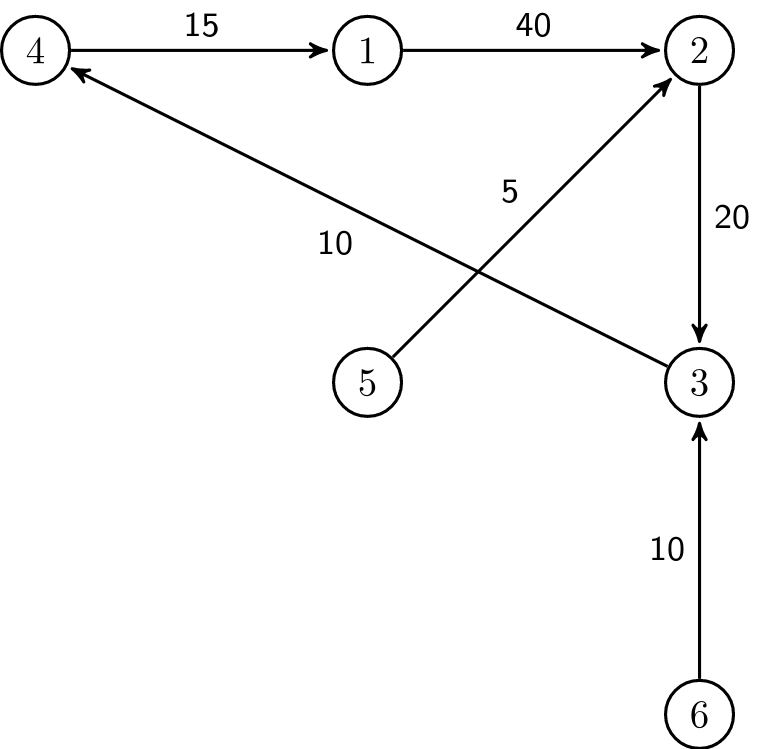
\includegraphics[scale=0.15]{imagenes/ejemplo2.png}

\end{minipage}

\bigskip

Como vemos, la única manera de salir de una ciudad y volver a la misma es que arranquemos en las ciudades 1, 2, 3 ó 4, y recorramos las cuatro rutas que las conectan. Por ende, debemos asegurar que al recorrerlas no se le saca plata al estado; es decir, que al aplicarle el subsidio fijo, se descuenta menos de (40+20+10+15) $=$ 85 pesos. Considerando que las cuatro rutas tienen el mismo descuento, el mayor subsidio que se podría realizar es la cuarta parte de 85, que si lo redondeamos es 21 pesos. Por lo tanto, el mayor descuento que se podría realizar a las rutas de esta provincia es de 21 pesos.

\subsection{Desarrollo}
Dado este problema, y considerando que hay que tener en cuenta la mano en la cual corren las rutas, la mejor manera de modelarlo sería utilizando digrafos. Así, cada ciudad se representaría con un nodo, y cada una de las rutas que conecta dos ciudades, con una arista dirigida. Consideraremos que un recorrido abusivo es representado por un ciclo negativo en el digrafo.

Como nuestro problema principal es averiguar cual es el mayor subsidio que se le puede otorgar a todas las rutas sin que se generen ciclos de rutas negativos, no es dificil que rápidamente encontremos una visión certera de lo que debemos hacer en el problema. Como primer aproximamiento, podemos asegurar que nuestro objetivo será reducir el costo de las rutas de manera que vayamos obteniendo mejores valores hasta que, superado el valor máximo, encontremos ciclos negativos en nuestro grafo.

Por ende, sabemos de entrada que necesitaremos un algoritmo capaz de reconocer ciclos negativos; y considerando los límites de complejidad brindados, podemos asegurarnos que Bellman-Ford cumple nuestros propositos. Esto nos permitirá utilizar aristas negativas, y averiguar en cada uno de los nodos si en sus componentes hay o no ciclos negativos.

Dado que en el problema original queremos detectar la existencia de ciclos negativos para distintas versiones del mismo grafo, usamos una función que permite crear una nueva versión del grafo a partir del original. Diremos que una p-versión nueva del grafo contiene la misma cantidad de nodos y representa al mismo conjunto de adyacencias, y su diferencia radica en que para todo eje de u a v con peso w perteneciente al grafo original, hay un eje de u a v con peso (w-p) perteneciente a la p-versión. Así, utilizaremos un algoritmo que, para cada versión, nos diga si efectivamente al aplicarle Bellman Ford se encuentran o no ciclos negativos (para esto, suponemos que Bellman-Ford nos devuelve $true$ si encuentra ciclos negativos, y $false$ si no lo hace)

\begin{algorithm}[H]
	\NoCaptionOfAlgo
	\caption{\algoritmo{ajusteParaBellmanFord}{\In{p}{int}, \In{ejesGrafo}{lista[ejes]}, \In{origen}{int}}{bool}}
	
	lista[ejes] ejesPVersion $\leftarrow$ ajustarEjes(ejesGrafo, p)

	res $\leftarrow$ bellmanFord(ejesPVersion, origen)
\end{algorithm}

Diremos que c es el peso de la arista mas pesada del grafo original. Veamos que la versión p $=$ 0 es equivalente al grafo original, y por ende no puede tener ciclos negativos. Por otro lado, veamos que si el grafo original tiene ciclos, la versión p $=$ c + 1 tendrá ciclos negativos, porque todas sus aristas serán negativas. Por ende, sabemos que nuestra solución esta acotada inferiormente por 0 y superiormente por c.

Por otro lado, teniendo en cuenta un Q cualquiera, sabemos que si la versión Q carece de ciclos negativos entonces toda versión con un valor de subsidio menor a Q también carecerá de ellos. La intuición aquí reside en notar que aumentar el peso de cada arista de un grafo sin ciclos negativos producirá el aumento del peso del ciclo, y por lo tanto, que se mantenga por arriba de 0. Y del mismo modo, podemos notar lo inverso: si la versión Q posee ciclos negativos, toda versión con un valor de subsidio mayor a Q los contendrá.

Entonces, sabiendo que un valor Q bien nos habla de todos los mayores o menores a él; y considerando que nuestra solución se encuentra entre 0 y c, podemos realizar una búsqueda binaria tal que para cada versión Q, si la misma posee ciclos negativos, nuestra solución se acotará entre 0 y Q. En cambio, si no los posee, su solución se encontrará entre Q y c.

Dado que Bellman-Ford parte de un nodo s y actualiza las distancias entre s y el resto de los nodos, solo puede detectar ciclos negativos si estos pertenecen a la misma componente conexa que s. Si el grafo G de entrada no es conexo, no existe nodo de partida que sirva para reconocer a todas las componentes de G. Proponemos la creación de un nodo con $d_{out} = n \land d_{in} = 0$. En otras palabras para todo nodo v perteneciente a G, existe un eje que va de s a v. Ahora el algoritmo de Bellman-Ford puede utilizar a s como nodo de partida y tenemos garantizado que podremos reconocer todos los ciclos negativos. Acabamos de agregar un nodo y n aristas, con lo cual la complejidad nos queda $O((n+1)*(n+m)) \in O(n^2+n*m)$ como por hipótesis, todo nodo v perteneciente a G cumple que $d_{out}(v) > 0$ vemos que $n \leq m$ y por lo tanto $O(n^2+n*m) \in O(n*m)$ osea que al agregar a s y sus ejes, la complejidad no empeora.

Finalmente, nuestro algoritmo definitivo itera de manera binaria, lo cual nos da un ciclo que se recorre $O(log(c))$ veces para la complejidad $O(n.m)$, dándonos, en definitiva, una cota temporal de $O(n.m.log(c))$

\subsection{Experimentacion}

La experimentación de este ejercicio representó un desafío, ya que en la generación de grafos resultó difícil garantizar condiciones que diesen resultados homogéneos debido a nuestra implementación. Esto requeriría crear grafos fuertemente conexos, de modo que ningún eje estuviese fuera de un ciclo. Sin embargo, sí pudimos observar fácilmente los casos de grafos completos.

\begin{center}
	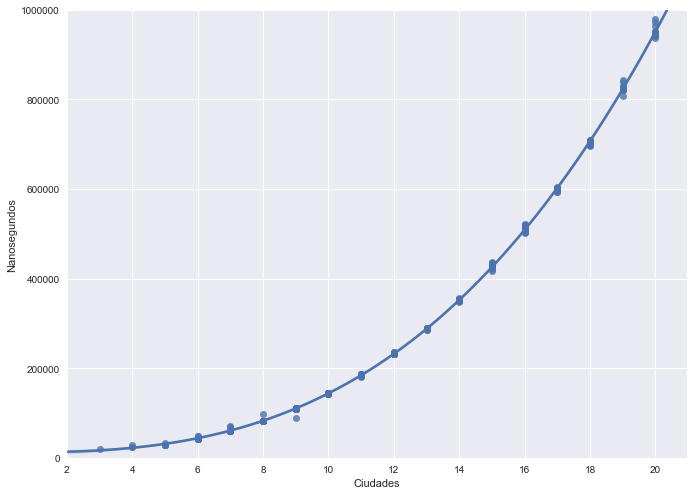
\includegraphics[scale=0.5]{imagenes/ej2-1.png}
\end{center}

En este gráfico se puede observar que, en grafos completos, el algorítmo tiene complejidad cúbica con respecto a la cantidad de ciudades. Esto se ajusta a la complejidad pedida, ya que $m = \frac{n \times (n-1)}{2} \approx n^2$, es decir, $O(n m) \subseteq O(n^3)$.

\begin{center}
	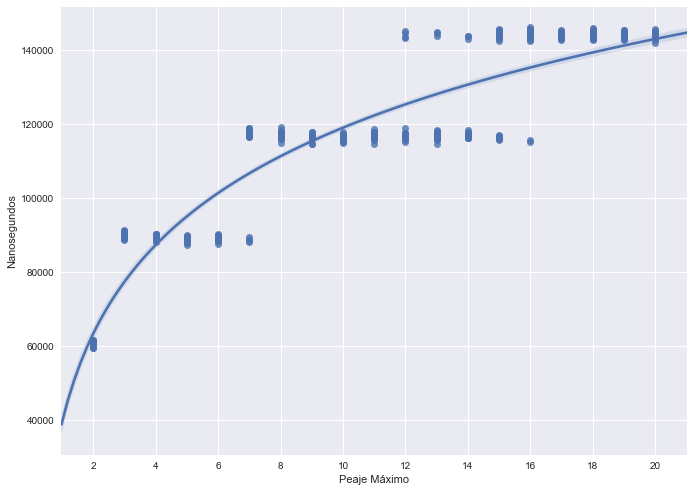
\includegraphics[scale=0.5]{imagenes/ej2-2.png}
\end{center}

Por otro lado, podemos ver que el máximo peaje tiene impacto logarítmico sobre el tiempo de ejecución, lo que condice con nuestras expectativas y con la cota de complejidad pedida.

\section{Reconfiguración de rutas}

\subsection{Descripción del problema}
Este problema plantea otra provincia de provincia de Optilandia, en la cual, sus ciudades están conectadas por rutas, aunque tiene unos problemas, algunas ciudades no están conectadas y hay otras de la cual se puede viajar de una a la otra de varias maneras. 
Para solucionarlo, el gobierno hará obras en las rutas para que haya una y sólo una forma de llegar desde cualquier ciudad a otra, construyendo nuevas rutas o destruyendo rutas rutas existentes.
\\
\par
Nos piden un algoritmo que dado las rutas y los costos de construcción y destrucción, nos de que rutas hay que destruir y construir para satisfacer el problema de forma que gastemos lo menor posible, como requisito la complejidad de este algoritmo no puede ser peor que \textbf{O($n^2log(n)$)}, donde n es la cantidad de ciudades de la provincia.
\\
\par
\textbf{Agregar ejemplos}
\\
\par
\subsection{Desarrollo}

\subsection{Cota temporal}

\subsection{Experimentacion}

\pagebreak

% compilar 2 veces para actualizar las referencias


\end{document}